\chapter{Gr\"obner-basis engines}\label{sec:groebner}

Before root finding, the decomposition oracle was a Gr\"obner solve, and
for $m\ge3$ over binary fields it still is. The repository grew a family
of engines (\art{docs/ic/GROEBNER_F4F5F6_AUDIT_20261010.md}, \S1; file names below are under \art{src/cryptanalysis/}):

\begin{description}[style=nextline, leftmargin=1.4em]
\item[Matrix F4 and F5 over $\FF_2$] (\art{koblitz_groebner.rs},
  \art{matrix_f5_f2.rs}): Macaulay matrices of the Weil-restricted Boolean
  system, reduced by a shared Four-Russians kernel (\art{gf2_elim.rs}, four
  8-bit tables, AVX-512 or AVX2).
\item[Inherited F4] (\art{inherited_f4.rs}, from 22 September, the
  default algebraic oracle): a DPLL-style tree over partial assignments in
  which each child \emph{inherits} its parent's echelon form and re-reduces
  only what the assignment changed, instead of building a fresh Macaulay
  matrix per node.
\item[F6-IC] (opt-in): inherited F4 plus a factor-base domain gate (a
  fully assigned summand whose abscissa is not a base point refutes;
  partial support pruning refutes earlier), and meet-in-the-middle leaves
  (with $m-1$ summands fixed the last is looked up; at $m=3$ and
  $\abs\Fb\le256$ every compatible second point is added and the third
  looked up).
\item[$\FF_p$ F4] (\art{f4_fp.rs}, \art{f4_fp_tower.rs},
  \art{sig_fp_tower.rs}): degree-bounded F4 with sparse-by-reducer then
  dense reduction, a Faug\`ere--Lachartre block for the Kummer-tower
  oracle, and a signature variant.
\end{description}

\paragraph{Correctness.} The audit pinned every engine against every
other and against brute force (88+15+9+14+13+12+21+6 passing library
tests in the touched modules), and found one soundness bug
(\S\ref{sec:corrections}, item 6), two contract defects and several latent
holes, all fixed with regression tests.

\paragraph{Engineering results.} Figure~\ref{fig:engine} collects the
headline ratios and Table~\ref{tab:prog_groebner-engineering} lists them
all; all are \cls{engineering} with identical outputs.

\begin{table}[p]
\centering\footnotesize
\begin{tabular}{@{}>{\raggedright\arraybackslash}p{0.27\linewidth}>{\raggedright\arraybackslash}p{0.2\linewidth}>{\raggedright\arraybackslash}p{0.2\linewidth}>{\raggedleft\arraybackslash}p{0.2\linewidth}@{}}
\toprule
Change & Case & Measure & Ratio or value \\
\midrule
Matrix / inherited F4 & K13 & counted matrix work & $198.6\times$ \\
 & random-13 & & $222.1\times$ \\
 & $m=19$ & wall, matrix F4/F5 vs inherited F4 & timed out at 1{,}800\,s vs about 6\,s \\
\addlinespace
F5 / F4 & K13 & word XORs & $0.6465$ \\
 & random-13 & & $0.6414$ \\
 & K13, random-13 & wall & $0.79$--$0.86$ \\
\addlinespace
F6-IC / inherited F4 & $m=13$ & word XORs & about $0.82$ \\
 & $m=19$ & & $0.77$--$0.78$ \\
 & --- & relation wall & $1.7$--$1.9\times$ faster \\
 & $m=13$ & $S$, group additions charged & $64.6$--$68.8\times$ \\
 & $m=19$ & & $1{,}303$--$1{,}353\times$ \\
 & K13 & $S$, word XORs priced (\#1774) & $1{,}572.1/634.12\approx2.5\times$ \\
 & R13, $m=19$ & & lower bounds \\
 & $m=31$ & first target & both hit 3{,}600\,s cap \\
\addlinespace
Every echelon call to the Four-Russians kernel & oracle's own Macaulay matrices & speed-up & $1.75$--$3.22\times$ \\
Word-level \texttt{pext}/\texttt{pdep} rewrite plan & $n=23$ & F4 and F6-IC faster & 10--14\% \\
Eager / lazy rewrite of kept rows & & speed-up & $1.40$--$1.62\times$ \\
\addlinespace
Fused construction and readback & F4 & instructions & $-5.28\%$ \\
 & F5 & & $-11.02\%$ \\
Native hashing & F5 & & $-3.715\%$ $[3.714,3.726]$ \\
 & standalone criterion & & $-45.1\%$ \\
Bounded direct indexing in the F5 packer & F5 & & $-3.947\%$ \\
Row allocation & & requested bytes & $42$--$50\%$ fewer \\
\addlinespace
Quotient-curve model / symmetrised control & $m=2$, five interleaved cells & F4 word operations cut & $1.340$--$1.642\times$ \\
\addlinespace
Branchless AVX2 strip & one thread & speed-up & $1.210\times$ \\
Bitmap seen-set in Boolean F4 & full F4 & & $1.199\times$ \\
Combined F5 options & & & $1.530\times$ \\
Fixed support cut & one complete call & & $3.02$--$3.07\times$ \\
Graded reuse in F5 & & & $1.78$--$1.84\times$ \\
\addlinespace
\texttt{f4\_fp} / its predecessor & square generic systems & speed-up & $29.8$--$54.1\times$ \\
msolve / ours & single-threaded & ratio & $0.96$--$1.22$ \\
Ours / msolve, blocked pair reduction & two largest square systems & time & $0.75$--$0.78\times$ \\
 & four others & & $1.11$--$1.49\times$ \\
msolve faster, a day earlier & & time & $12$--$24\times$ \\
Boolean decomposition systems, $n=17$, 8 targets & our oracle (decides) & time per target & 7--24\,ms \\
 & msolve, PolyBoRi (full basis) & & 40--52\,s \\
 & Singular & & exceeds 120\,s \\
\bottomrule
\end{tabular}
\caption[]{Gr\"obner-engine engineering results, all \cls{engineering}
with identical outputs. \emph{Change}: candidate / baseline where a slash
is shown; \emph{Case}: target set or size (K13, random-13 and R13 as named
in the sources; $m$ the number of summands; ``---'': no
case given); \emph{Measure}: the counted or timed quantity; \emph{Ratio or
value}: as recorded. Groups, top to bottom, with sources: inherited versus
matrix F4 (\art{research/f4_f5_f6_cross_family_20261011/}); F5 versus F4;
F6-IC versus inherited F4 (priced and lower-bound cells:
\art{research/f4_pricing_jump_20261018/}); kernel routing and rewrite
(\art{research/inherited_f4_eager_rewrite_20261011/}); instruction and
allocation work, by paired A/B/A$'$ instruction counts on a frozen
eleven-system suite, elapsed time not claimed; the quotient-curve model
(\art{research/lit2026_w8_summation_models_20261011/}); $\FF_2$ campaign
results (strip: \art{research/gf2_branchless_strip_20260929/}; seen-set:
\art{research/boolean_f4_bitmap_20260926/}; combined options:
\art{research/f5_combined_2x_20260928/}; support cut:
\art{research/f5_support_cut19_confirm_20261003/}; graded reuse:
\art{research/boolean_f5_graded_batch_20261002/}); $\FF_p$ F4 to msolve
parity (\art{research/f4_fp_msolve_parity_20261011/}; blocked pairs:
\art{research/f4_fp_blocked_pairs_20261016/}; the day-earlier msolve
reading: \art{research/gb_cas_comparison_20261011/}).}
\label{tab:prog_groebner-engineering}
\end{table}

Matrix and inherited F4 can return different decompositions, so their
splitting trees may differ; only matrix F4 and F5 share a tree by
construction. F6-IC's $S$ ratios, once its batched group additions are
charged, are an accounting loss, not a frontier move. Those ratios used
inherited F4 before its word XORs were priced (\#1774); priced, F6-IC is
still a loss at K13, while the R13 and $m=19$ cells remain lower bounds.

The $\FF_2$ engine campaigns (about 90 directories, 22 September--17
October; the programme record~\cite{icprogram2026}, clusters ``boolean'',
``gf2-elim'', ``f5-kernel'', ``f5-support-cut'', ``f4-f5-shared'') gated
each micro-change against the strongest reference, and most failed. Kept as
defaults: the branchless strip, the bitmap seen-set, batched pair inserts,
five-column tables, and direct packing in F5 (default since 17 October).
About thirty unpack, pivot, layout and packing variants were refuted, and
graded reuse in F5 fell short of the campaign's $2\times$ goal. These are
stage speed-ups of the decision engine; none changes an index-calculus
distance to rho. Every reduced basis of \texttt{f4\_fp}, after
Gebauer--M\"oller criteria, packed monomials, interned symbolic
preprocessing and a parallel symbolic pass, agrees with Singular or msolve.
The Boolean comparison is a difference of task (decide versus compute the
basis), not of engine quality.

\begin{figure}[t]
\centering
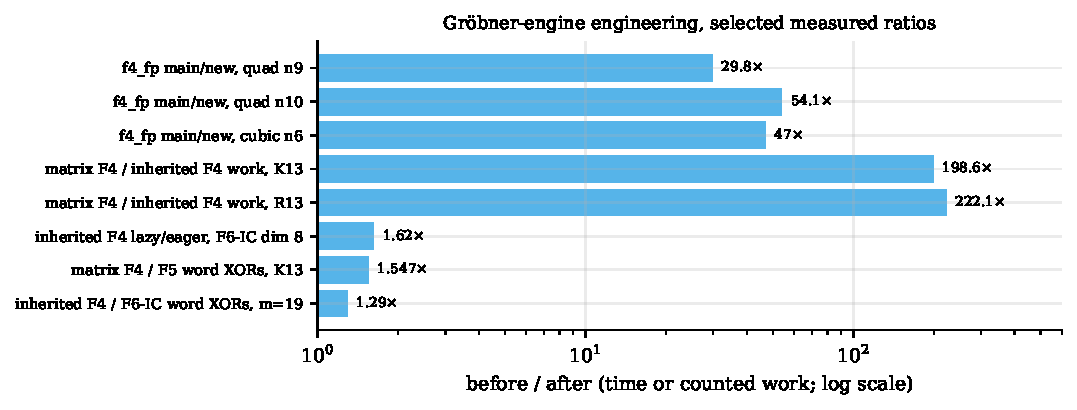
\includegraphics[width=\linewidth]{figures/fig-engine.pdf}
\caption[]{Selected engine ratios (before/after or baseline/candidate):
\texttt{f4\_fp} successive versions (single-threaded wall, L0); matrix
versus inherited F4 (counted matrix work); lazy versus eager inherited
rewrite (median wall); F4 versus F5 and inherited F4 versus F6-IC (word
XORs, stage only). Sources in \art{figures/data-program.json}.}
\label{fig:engine}
\end{figure}

\paragraph{What did not work.} Degree-2 early-abort probes after a
2025--26 proposal: word-XOR ratios $1.00083$--$1.00378$ (no change) and
$0.99714$--$0.99928$ (worse). Gate-first geometry: $1.57$--$1.78\times$
fewer word XORs but lane-batched F4 roots cost $2.6$--$4.0\times$ a
sequential control. Convolution splitting of the summation polynomial:
$1.21$--$2.07\times$ \emph{more} word operations despite lower degree;
Frobenius auxiliary variables: $57$--$701\times$ more
(\art{research/lit2026_w\{4,5,8\}_*_20261011/}). Symmetry-breaking clauses
in SAT did not help (\art{RESEARCH_KOBLITZ_INDEX_CALCULUS.md}). A
registered law for the $m=3$ refutation degree resolved all 68 units but
ended with the verdict ``neither'': one variant met its generic degree
window on 32/32 draws, the other fell below it on 8, and the heaviest
degree-10 Macaulay solves were $2.4\cdot10^5\times2.0\cdot10^5$ matrices at
42--51 minutes each (\art{research/ic_semiregular_law_20261005/}).
